\section{Data Collection}
The experimental data for this project was collected using an \textbf{iPhone 13}, equipped with a dual-camera system (wide and ultra-wide lenses). Specifically, the main wide-angle lens was selected due to its superior optical properties and stability in low-light conditions. The video was recorded in an urban environment, capturing moving vehicles at nighttime to reflect the conditions targeted by this study.

The camera was mounted on a stable tripod at a fixed position and inclination, approximately 2.5 meters above the ground, ensuring a clear and consistent perspective of the roadway. The distance from the camera to the road was approximately 10 meters, providing sufficient perspective to capture clear geometric features on the vehicle.

The recording settings chosen were:
\begin{itemize}
    \item Resolution: $3840 \times 2160$ pixels (4K)
    \item Frame rate: 30 frames per second
    \item Exposure: Automatic (AE lock enabled), optimized for nighttime recording
    \item Focus: Automatic (AF lock enabled)
    \item Format: HEVC (High Efficiency Video Coding)
\end{itemize}

It is important to note that if AE (auto-exposure) and AF (auto-focus) are not locked during video capture, the camera may continually adjust exposure and lens focus. Exposure variations (such as ISO or shutter speed) do not alter the camera's intrinsic matrix, which is determined by the focal length and optical center. However, autofocus can induce physical movement of the lens elements, slightly changing the effective focal length through a phenomenon known as lens breathing. This may introduce per-frame variations in the intrinsic matrix. Therefore, in applications requiring a stable calibration—such as precise vehicle localization using geometric constraints—it is strongly recommended to lock both AE and AF during video acquisition to maintain consistency.

\section{Camera Calibration}
Accurate camera calibration is crucial for the geometric computations required by this project. In order to collect as many calibration frames as possible, we recorded a video of the checkerboard using the exact same camera settings applied during vehicle capture. From this video, 99 frames were extracted showing the checkerboard from various angles and distances, ensuring robust input for calibration. This approach helped to improve the numerical stability and accuracy of the intrinsic parameter estimation. To obtain the camera's intrinsic parameters (the K matrix), a standard calibration procedure was implemented. A calibration pattern (a planar chessboard with known dimensions: square size of 24.5mm) was used, capturing multiple images at varying angles and distances from the camera.

Calibration was initially performed using custom Python code, leveraging OpenCV functions (cv2.findChessboardCorners, cv2.calibrateCamera). To ensure accuracy and reliability, the resulting intrinsic parameters were cross-validated using the iOS Camera API, specifically leveraging metadata provided by the AVCaptureDevice API. This API reports intrinsic parameters computed internally by iOS during video recording.

The computed intrinsic matrix  obtained from our custom calibration procedure was:
\begin{equation}
    K = \begin{bmatrix}
        f_x & 0 & c_x \\
        0 & f_y & c_y \\
        0 & 0 & 1
    \end{bmatrix} =
    \begin{bmatrix}
        3.20149890e+03 & 0 & 1.93982925e+03 \\
        0 & 3.20637527e+03 & 1.06315413e+03 \\
        0 & 0 & 1
    \end{bmatrix}
\end{equation}

Additionally, the calibration process also produced the following distortion coefficients:
\begin{equation}
    \text{Distortion coefficients: } \begin{bmatrix}
        2.43773846e-01 \\
        -1.59544680e+00 \\
        -1.15284213e-03 \\
        4.19886247e-04 \\
        3.56681588e+00
    \end{bmatrix}
\end{equation}

Moreover, the calibration process resulted in a root mean square (RMS) reprojection error of:
\begin{equation*}
    \text{RMS Reprojection Error: } 0.7705
\end{equation*}

The root mean square reprojection error of 0.7705 pixels confirms the accuracy and consistency of the intrinsic parameters obtained, particularly considering the smartphone camera context and the use of diverse viewpoints.

Cross-checking these parameters with those provided by the AVCaptureDevice API yielded some noticeable differences. The matrix obtained from the iOS API was:
\begin{equation}
    K_{\text{API}} =
    \begin{bmatrix}
    2805.4324 & 0 & 1919.5735 \\
    0 & 2805.4324 & 1077.1753 \\
    0 & 0 & 1
    \end{bmatrix}
\end{equation}

While this matrix appears significantly different in focal length values, we believe it may reflect internal lens parameterizations not directly influenced by real-world geometry or may be affected by system-level post-processing. Given that our OpenCV-based calibration was performed using real scene images and yielded consistent reprojection errors, we consider our computed matrix more reliable for geometric reasoning tasks.

\begin{figure}[htbp]
    \centering
    % Top row: two subfigures side by side
    \begin{subfigure}[b]{0.48\textwidth}
        \centering
        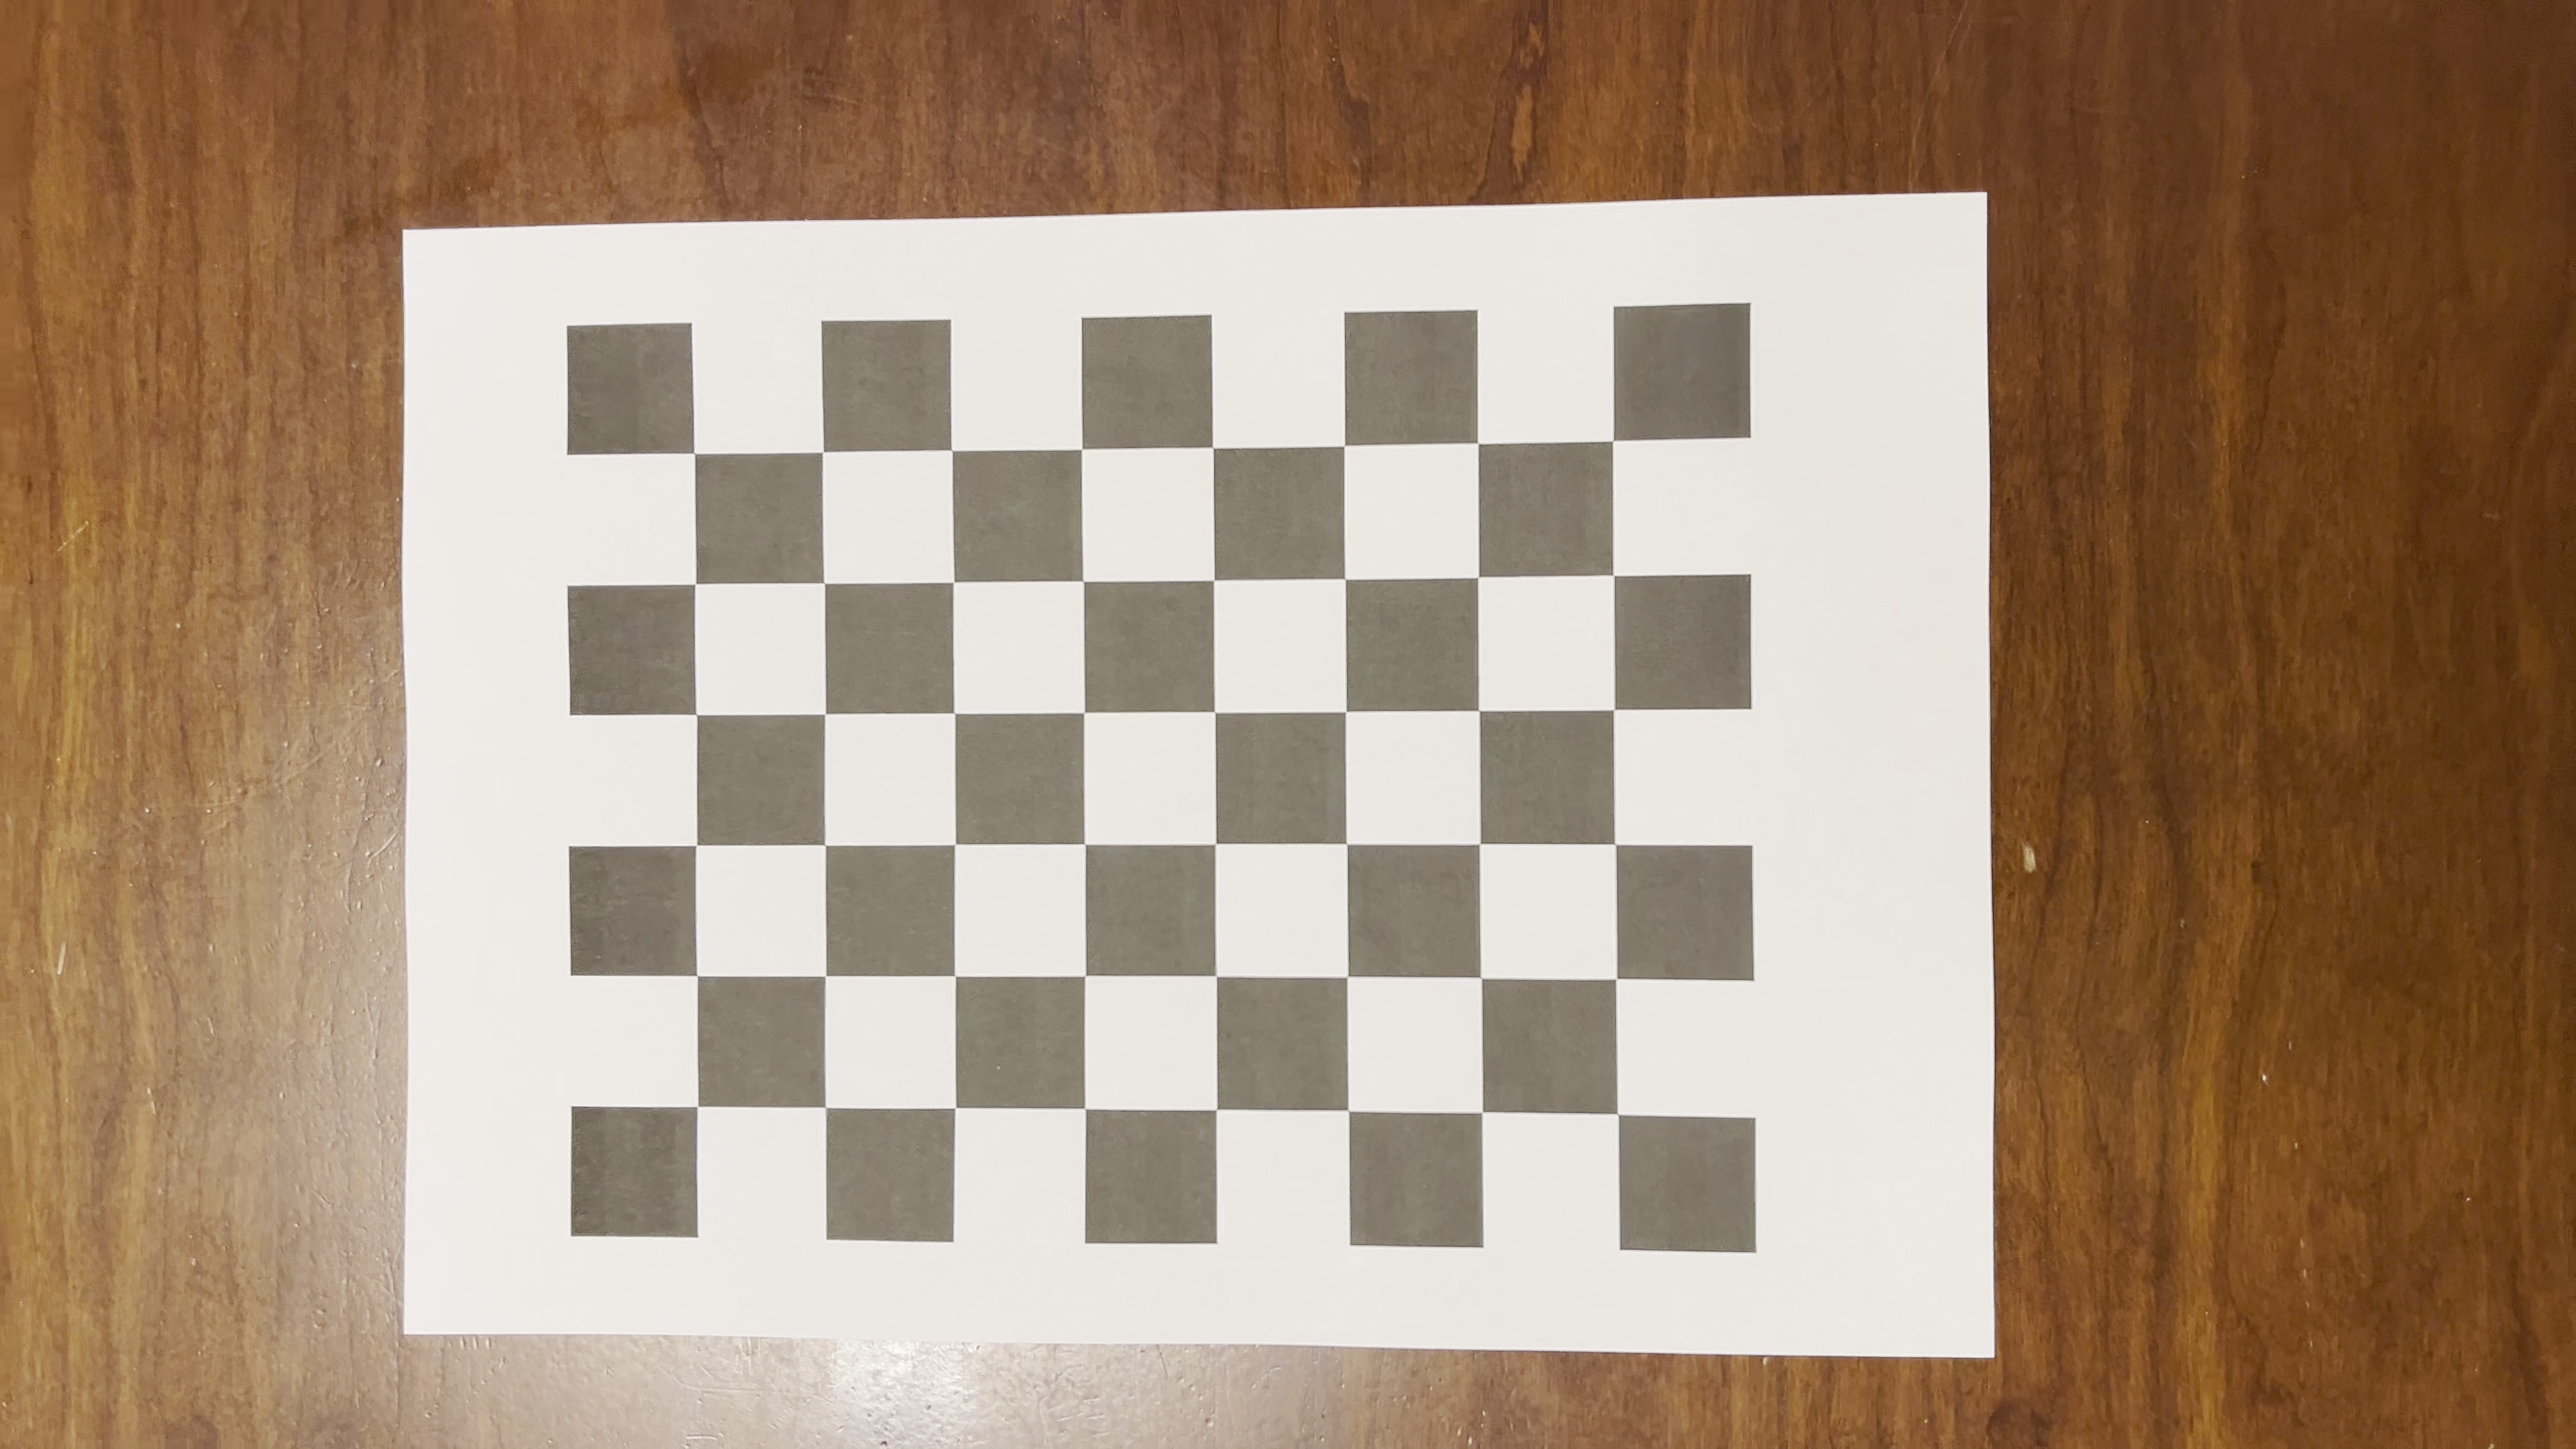
\includegraphics[width=\textwidth]{Images/checkerboard_frame_raw.png}
        \caption{Checkerboard corners detected using \texttt{cv2.findChessboardCorners}.}
        \label{fig:checkerboard-raw}
    \end{subfigure}
    \hfill
    \begin{subfigure}[b]{0.48\textwidth}
        \centering
        \includegraphics[width=\textwidth]{Images/checkerboard_frame_annotated.png}
        \caption{Detected corners annotated on frame.}
        \label{fig:checkerboard-annotated}
    \end{subfigure}

    \vspace{1em} % adjust spacing between rows

    % Bottom row: montage image
    \begin{subfigure}[b]{0.85\textwidth}
        \centering
        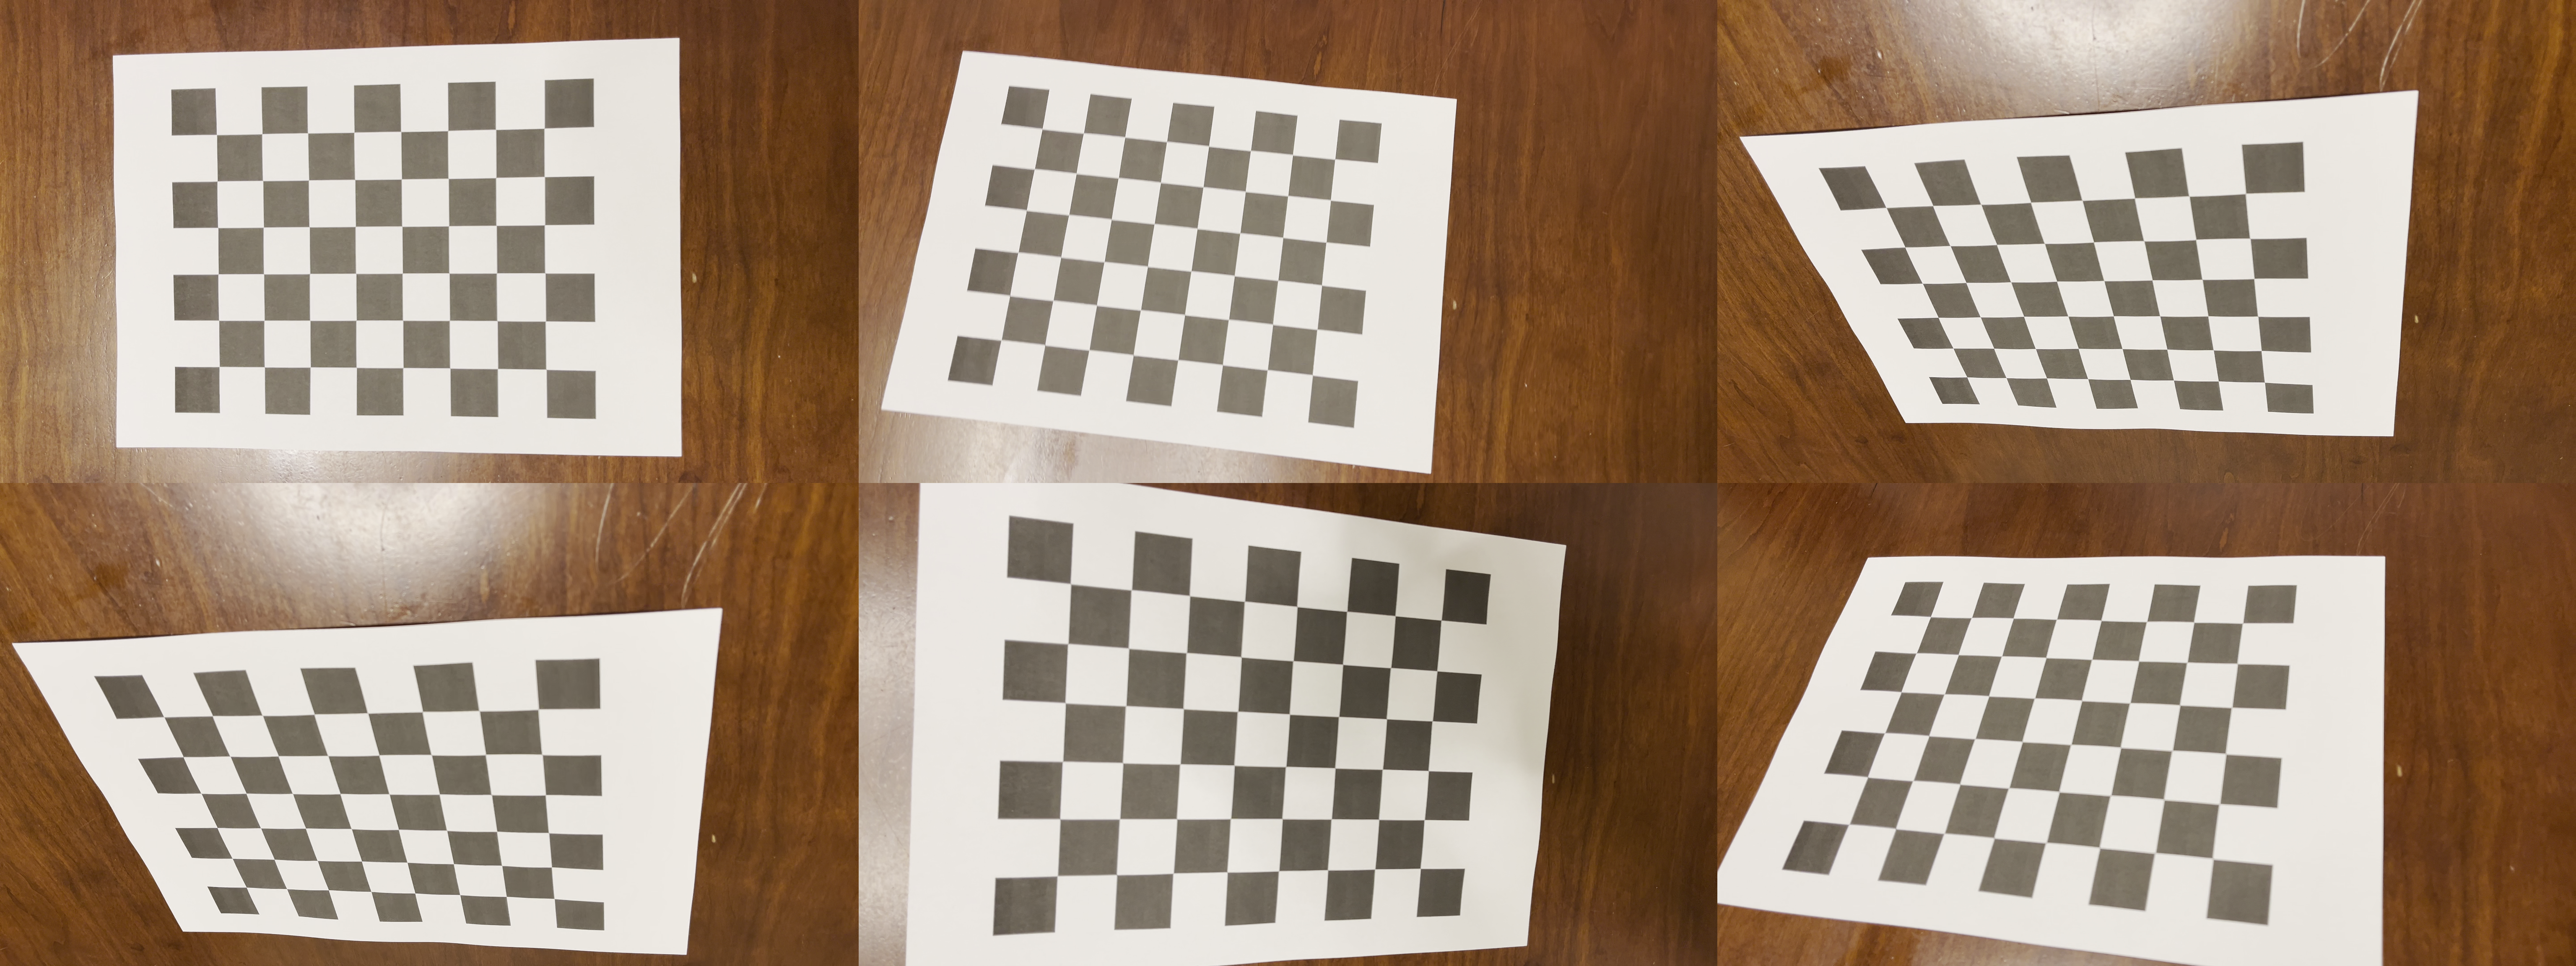
\includegraphics[width=\textwidth]{Images/checkerboard_montage.png}
        \caption{Multiple calibration views for geometric diversity.}
        \label{fig:checkerboard-diverse}
    \end{subfigure}

    \caption{Detected checkerboard corners (top) and selection of calibration frames (bottom).}
    \label{fig:checkerboard-combined}
\end{figure}

\section{Vehicle Model and Reference Dimensions}
The vehicle used as the reference model in this project is the \textbf{Škoda Fabia}. Its rear geometry was selected due to its clear symmetry, availability of technical dimensions, and suitability for feature-based pose estimation. All geometric measurements, including the positions of rear lights, license plate corners, and mirrors, were manually extracted from the official reference image and scaled to millimeters.

The following are the main physical dimensions used:

\begin{itemize}
    \item \textbf{Height of internal rear lights (A–B)}: 1000 mm
    \item \textbf{Height of external rear lights (E–F)}: 1200 mm
    \item \textbf{Height of license plate lower corners (C–D)}: 900 mm
    \item \textbf{Width of the license plate (distance C–D)}: 520 mm
    \item \textbf{Distance between internal rear lights (A–B)}: 860 mm
    \item \textbf{Distance between external rear lights (E–F)}: 1400 mm
    \item \textbf{Total vehicle width (O–F)}: 1732 mm
    \item \textbf{Wheel-to-wheel width (O–O)}: 1457 mm
    \item \textbf{Angle $\varphi$ between the vertical and the rear surface of the vehicle}: $9.46^\circ$
\end{itemize}

\begin{figure}[htbp]
    \centering
    \includegraphics[width=0.85\textwidth]{Images/cad.jpg}
    \caption{2D CAD-style schematic of the reference vehicle (Škoda Fabia), annotated with labeled feature points and known dimensions in millimeters.}
    \label{fig:car-cad-model}
\end{figure}